\documentclass[a4paper]{article}

\usepackage[english]{babel}
\usepackage{amsmath}
\usepackage{graphicx}
%\usepackage{algorithm}
%\usepackage{algorithmic}
%\usepackage{algpseudocode}
\usepackage{url}


\title{Omega3P+PUMI Progress Report}

\author{Cameron W. Smith, Gerrett Diamond}

\date{\today}

\begin{document}
\maketitle
\section{Intro}

Unstructured mesh methods, like finite elements and finite volumes, support the
effective analysis of complex physical behaviors modeled by partial differential
equations over general three-dimensional domains.
The most reliable and efficient methods apply adaptive procedures with
a-posteriori error estimators that indicate where and how the mesh is to be
modified.
Although adaptive meshes can have two to three orders of magnitude fewer
elements than a more uniform mesh for the same level of accuracy, there are many
complex simulations where the meshes required are so large that they can only be
solved on massively parallel systems.

Parallel adaptive simulations repeatedly execute adaptive cycles composed of
steps.
Typically, the steps include pre-processing (preparing data structures for the
linear system construction), system assembly and solve, error-estimation,
adaptation.
Between each of these steps are opportunities to tune the distribution of the
data structures for higher performance.
For example, predictive load balancing can be performed prior to mesh adaptation
to reduce post adaptation imbalances and avoid memory exhaustion on parts with
heavy refinement.
Likewise, the time to completion for large scale system assembly and solve
procedures can be reduced by balancing the mesh entities holding
degrees-of-freedom can be balanced~\cite{SmithParma2015}.

Parallel simulations on massively parallel systems are most effective when data
movement is minimized.
Data movement costs increase with the depth of the memory hierarchy; a design
trade-off for increased capacity.
On modern processors the cost, in terms of peak bandwidth, of using the
filesystem instead of main memory is at least three orders of
magnitude~\cite{haring2012ibm,bui2014scalable}.
Software must leverage the cache and main memory bandwidth performance advantage
during as many operations as possible to maximize performance.

The Parallel Unstructured Mesh Infrastructure, PUMI
{\small (github.com/SCOREC/\\core)}~\cite{ibanez2015pumi},
provides in-memory mesh-based parallel simulations with mesh-adaptation, load
balancing, and tensor-field services.
Critical to the implementation of these services is the {\textit complete}
array-based~\cite{ibanezArray16} mesh representation.
This representation and its interface, APF, uses only a small amount of memory
(approximately 500B/element using 64 bit indices) and provides $O(1)$ mesh
adjacency queries.

The report begins by discussing techniques for in-memory software interactions
that avoid file I/O.
Section~\ref{sec:omega-pumi} then discusses our approach to Omega3P and PUMI
in-memory integration.
Next, Section~\ref{sec:parma} discusses the integration of the PUMI services
for static and dynamic load balancing in Omega3P.
Section~\ref{sec:software} briefly lists ACE3P software improvements.
Section~\ref{sec:results} concludes the report with closing remarks and next
steps.

\section{In-memory Integration}\label{sec:inmem}

We define a software component as a set of interfaces to query and modify
encapsulated state information.
The components in adaptive simulations that provide geometric model, mesh, and
field information~\cite{BeaWal,ibanez2015pumi,Ollivier10} are essential to error
estimation, adaptation, and load balancing~\cite{SmithParma2015} services.
Because of this strong dependency we package these components and services
together within the open-source PUMI~\cite{ibanez2015pumi} software.
Despite what the packaging may imply, the build system and interface design
minimizes the required set of dependencies for components that simply need to
query information, the use case for a typical finite element PDE solver.

Approaches for high performing and scalable component interactions avoid
file-based I/O through in-memory data streams and component functional
interfaces.
The ADIOS tools provide an alternative mechanism for the in-memory coupling of
executables~\cite{bennett2012combining,zhang2012enabling}; our work here focuses
on the interaction of libraries operating within the same process.
Components that support a common file format can use our data stream approach
with minimal software changes to exchange data via memory buffers instead of files.
This approach is also a logical choice for legacy analysis codes that do not
provide functional interfaces to access or create their input and output data
structures.

Components with functional interfaces that encapsulate creation, deletion, and
access to underlying data structures support in-memory interactions.
The level of interface granularity selected for defining interactions has a
proportional impact on flexibility and development costs.
At a very fine level a developer may implement all mesh entity query functions such
that components can share the same mesh structure; trading increased development
costs for lower runtime memory usage.
An excellent example of this is the use of octree structures in the
development of parallel adaptive analyses~\cite{BursteddeWilcoxGhattas11}.
At a coarser level a developer may simply create another mesh
representation through use of interfaces encapsulating mesh construction;
trading higher runtime memory usage for lower development costs.
For example, an existing solver component can embed low level
calls to mesh-entity iterators~\cite{Ollivier10}.
Although this method will allow for in-memory integration, it suffers from the
same disadvantages as a tightly coupled approach in that a significant amount of
time and effort will be required for code modification and verification.
A generalization of this coarser level approach defines common sets of
interfaces through which all components interact.
For example, in the rotorcraft aerodynamics community the HELIOS platform
provides a set of analysis, meshing, adaptation, and load balancing components
via the Python-based Software Integration Framework~\cite{sankaran2010application}.

\section{Omega3P+PUMI In-memory Integration}\label{sec:omega-pumi}

Omega3P is a C++ component within ACE3P for frequency analysis of linear
accelerator cavities.
It is built upon multiple components that include distributed mesh
functionality, tensor-field data management, vector and matrix math, and many
linear solvers.
Our in-memory integration of PUMI with Omega3P leverages these component interfaces to
execute mesh and tensor-field transformations (layout changes, data types, etc...) and 
transfers (copies).

The key advantage of this approach is the small amount of relatively simple code
required; we simply needed to read and write the Omega3P mesh and field structures.
However, an increase in peak memory usage will occur during the transfer when
there are two copies of the mesh and/or field data stored in memory.
Figure \ref{fig:memusage} shows the peak memory usage over the entire Omega3P
execution for both the original Omega3P code and with the PUMI mesh
(Omega3P+PUMI).
The increase in peak memory when storing the PUMI mesh is 2\% at 32 cores and
6\% at 128 cores.
At 32 cores there is a slight reduction in memory usage; we are still
investigating this.

\begin{figure}[ht]
\centering
  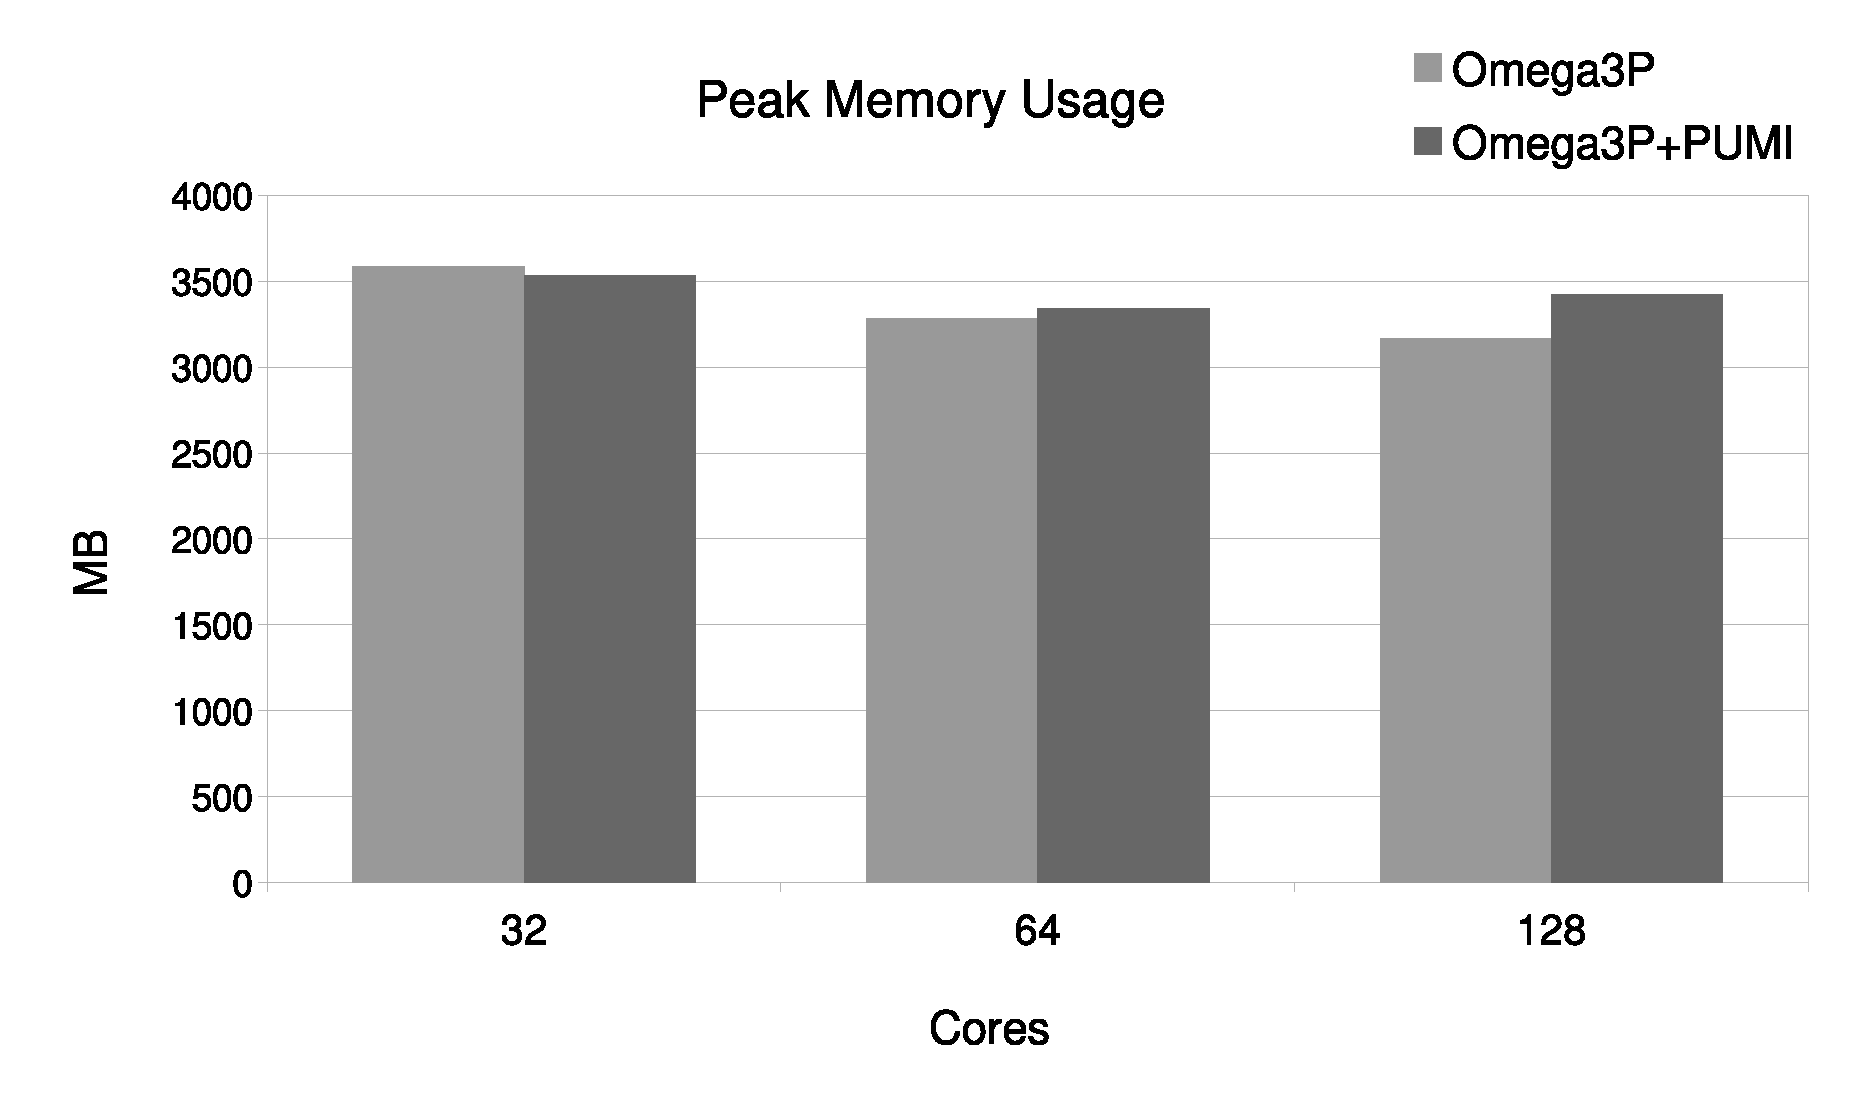
\includegraphics[width=\textwidth]{peak-memory-usage.eps}
  \caption{\label{fig:memusage} Peak memory usage. The labels above the Omega3P+PUMI bars
  list the percent increase versus Omega3P.}
\end{figure}

Mesh conversion begins with a version of Omega3P's NetCDF file reader that is altered
to read the mesh data into PUMI data structures instead of Omega3P's Distmesh. With 
the PUMI mesh we are able to perform partitioning and load balancing as well as adaptation 
while only storing the PUMI mesh. After we have a finalized PUMI mesh a second 
overloaded version of Omega3P's file reader is used to convert the PUMI mesh to 
Omega3P's DistMesh. This is done by using the data from the in-memory PUMI mesh as the 
input instead of the NetCDF file. After the conversion to DistMesh, we store both the
PUMI Mesh and the Omega3P DistMesh for the duration of the finite element setup and 
computations. The reading and converting of the mesh data together take less than 15\% 
of the total runtime and have a similar cost to the NetCDF read since the conversion
from PUMI to Distmesh is much faster than both the original file reading to Distmesh 
and the new file reading to PUMI. 

To support more efficient parallel workflows we have developed methods for
direct conversion of a curved parallel PUMI mesh to a curved parallel DistMesh and vice
versa.

\section{Load Balancing}\label{sec:parma}
ParMA, partitioning using mesh adjacencies, is a PUMI component that provides
multi-entity dynamic load balancing~\cite{SmithParma2015}.
ParMA's multi-entity balancing traverses an
application-specified priority list of entity orders (vertex, edge, face,
region) to balance in descending order.
For each entity order iterative diffusion is executed until balance is reached
or no further improvement is possible.
A diffusive iteration first determines which parts are imbalanced and which
neighboring parts, targets, can accept entities (weight) from them.
Next, a part-level graph distance heuristic is computed that measures how far each
boundary mesh element is from the parts topological center.
ParMA then iterates over the part boundary in descending order of distance to
select small sets of elements for migration.
The sets of boundary elements are selected if they are on the boundary with a
neighboring part that can accept weight, and if the migration would reduce the
weight of the sending part without increasing the number of entities on the
boundary (higher surface area).
Note, when a entity order of lower priority is being balanced ParMA will not disrupt
the balance of higher priority orders by accounting for the relative weight
difference during the selection of targets and boundary element
sets~\cite{SmithParma2015}.

ParMA's support for multi-entity balancing was extended for Omega3P's needs.
The Omega3P solving step relies on both on-part mesh entities as well as a layer
of ghosted elements along each part boundary.
Omega3P's ghosting uses vertex adjacency such that every element that shares a
vertex with a part boundary will be ghosted to each part that shares that
boundary.
This can be seen in Figure \ref{fig:ghost3} that shows an example of a mesh with
a layer of ghosting.
In order to improve Omega3P's performance and scalability, ParMA targets
minimizing the sum of the ghosted and on-part elements as well as the mesh
entities holding degrees-of-freedom.

\begin{figure}[ht]
\centering
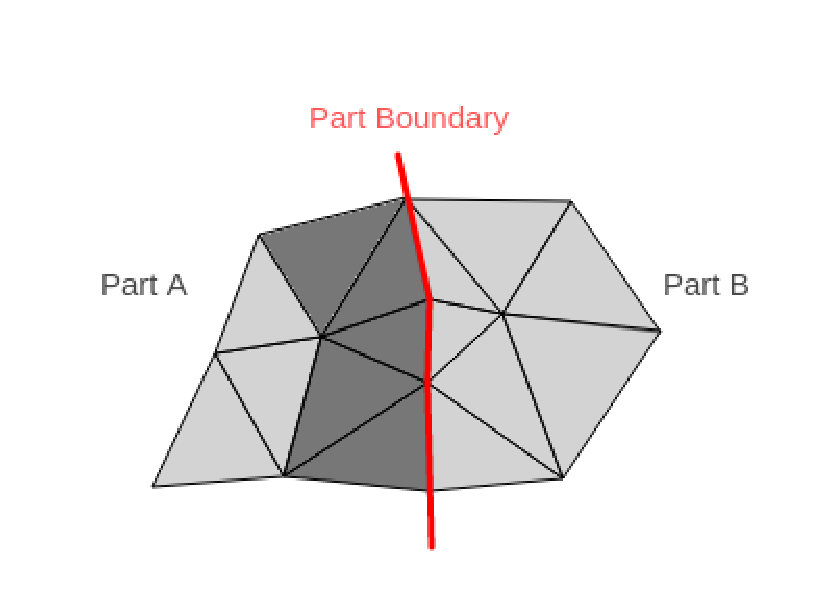
\includegraphics[width=0.8\textwidth]{ghost.eps} 
\caption{\label{fig:ghost3} A layer of ghosted elements from part A to part B. The darker elements represent all the elements on part A that part B will copy to create its remote mesh.}
\end{figure}

ParMA balances the degree-of-freedom holders defined by 
hierarchical Nedelec basis functions~\cite{ko2010advances,ingelstrom2006new} by
reusing existing multi-entity target and boundary-element selection
procedures.
For first order elements this requires balancing edges.
Second order elements requires edges and faces, and above that edges, faces, and
regions need to be balanced.
Each of these entity balancing procedures accounts for the ghosted weight
contribution by performing an additional neighborhood
exchange~\cite{ibanez2014hybrid} of the exact weight of ghosted layer entities.

\section{Software Status}\label{sec:software}
Our workflow currently supports reading a curved mesh from a NetCDF formatted file
into a DistMesh, or reading a PUMI mesh directly.
If a serial DistMesh was read it is converted to a PUMI-APF mesh and then 
partitioned using ParMETIS via the Zoltan interface.
Prior to running the Omega3P analysis the partition is balanced using ParMA
iterative diffusion methods.
ParMA diffusion directly modifies the distribution of the PUMI-APF mesh to
balance the degree of freedom holders and the ghosted mesh entities.
Lastly, prior to running the analysis, the PUMI-APF mesh is converted to
DistMesh.

During the development process the following software ACE3P software issues were
encountered:
\begin{itemize}
  \item The ACE3P Git repo contained a large collection of test data which
    results in a large download for developers.  Those files were moved to a
    privately shared directory prior to the creation of the private repo we have 
    been working in.
  \item The ACE3P Git repo contained the source code of
    external libraries it depends on.  In some cases the source code was modified.  
    We removed the external library source code from our private repo and documented 
    the versions needed and the exact changes required.
  \item The Boost-Build configuration on Cori and Edison used a combination 
    of pre-installed libraries and the libraries built from the ACE3P repo. We
    modified the boost-build configuration files to minimize the use of system
    libraries. Currently our build only depends on the system install of PetSC,
    netcdf, and the GNU Science Library (gsl).
  \item Calls to ParMETIS and Zoltan APIs were updated to support the latest
    versions, 4.0.3 and 3.81, respectively.
  \item We built ACE3P on the SCOREC Debian Jessie workstations.  This demonstrated 
    and exercised portability improvements and made the development process
    easier.
\end{itemize}

\section{Results and Next Steps}\label{sec:results}

We ran Omega3P and Omega3P+PUMI on the \texttt{cav17} model with a 318,118
element quadratic mesh on up to 128 cores (32 cores per node) of the NERSC Cori
Phase I system.
The Omega3P+PUMI average number of ghost + owned edges and faces per-part
is less than 1.46\% higher than the Omega3P counts at 32 parts.
At 64 and 128 parts the average entity counts of Omega3P+PUMI is less than 0.3\%
higher than Omega3P counts.
While maintaining nearly identical entity counts ParMA significantly reduces the
imbalance of ghost + owned elements and vertices. 
Figures~\ref{fig:vtx} and~\ref{fig:elm} respectively show the imbalance of
vertices and elements.
At 128 parts ParMA reduces the edge imbalance by 30 points and the face
imbalance by 27 points.

\begin{figure}[ht]
\centering
  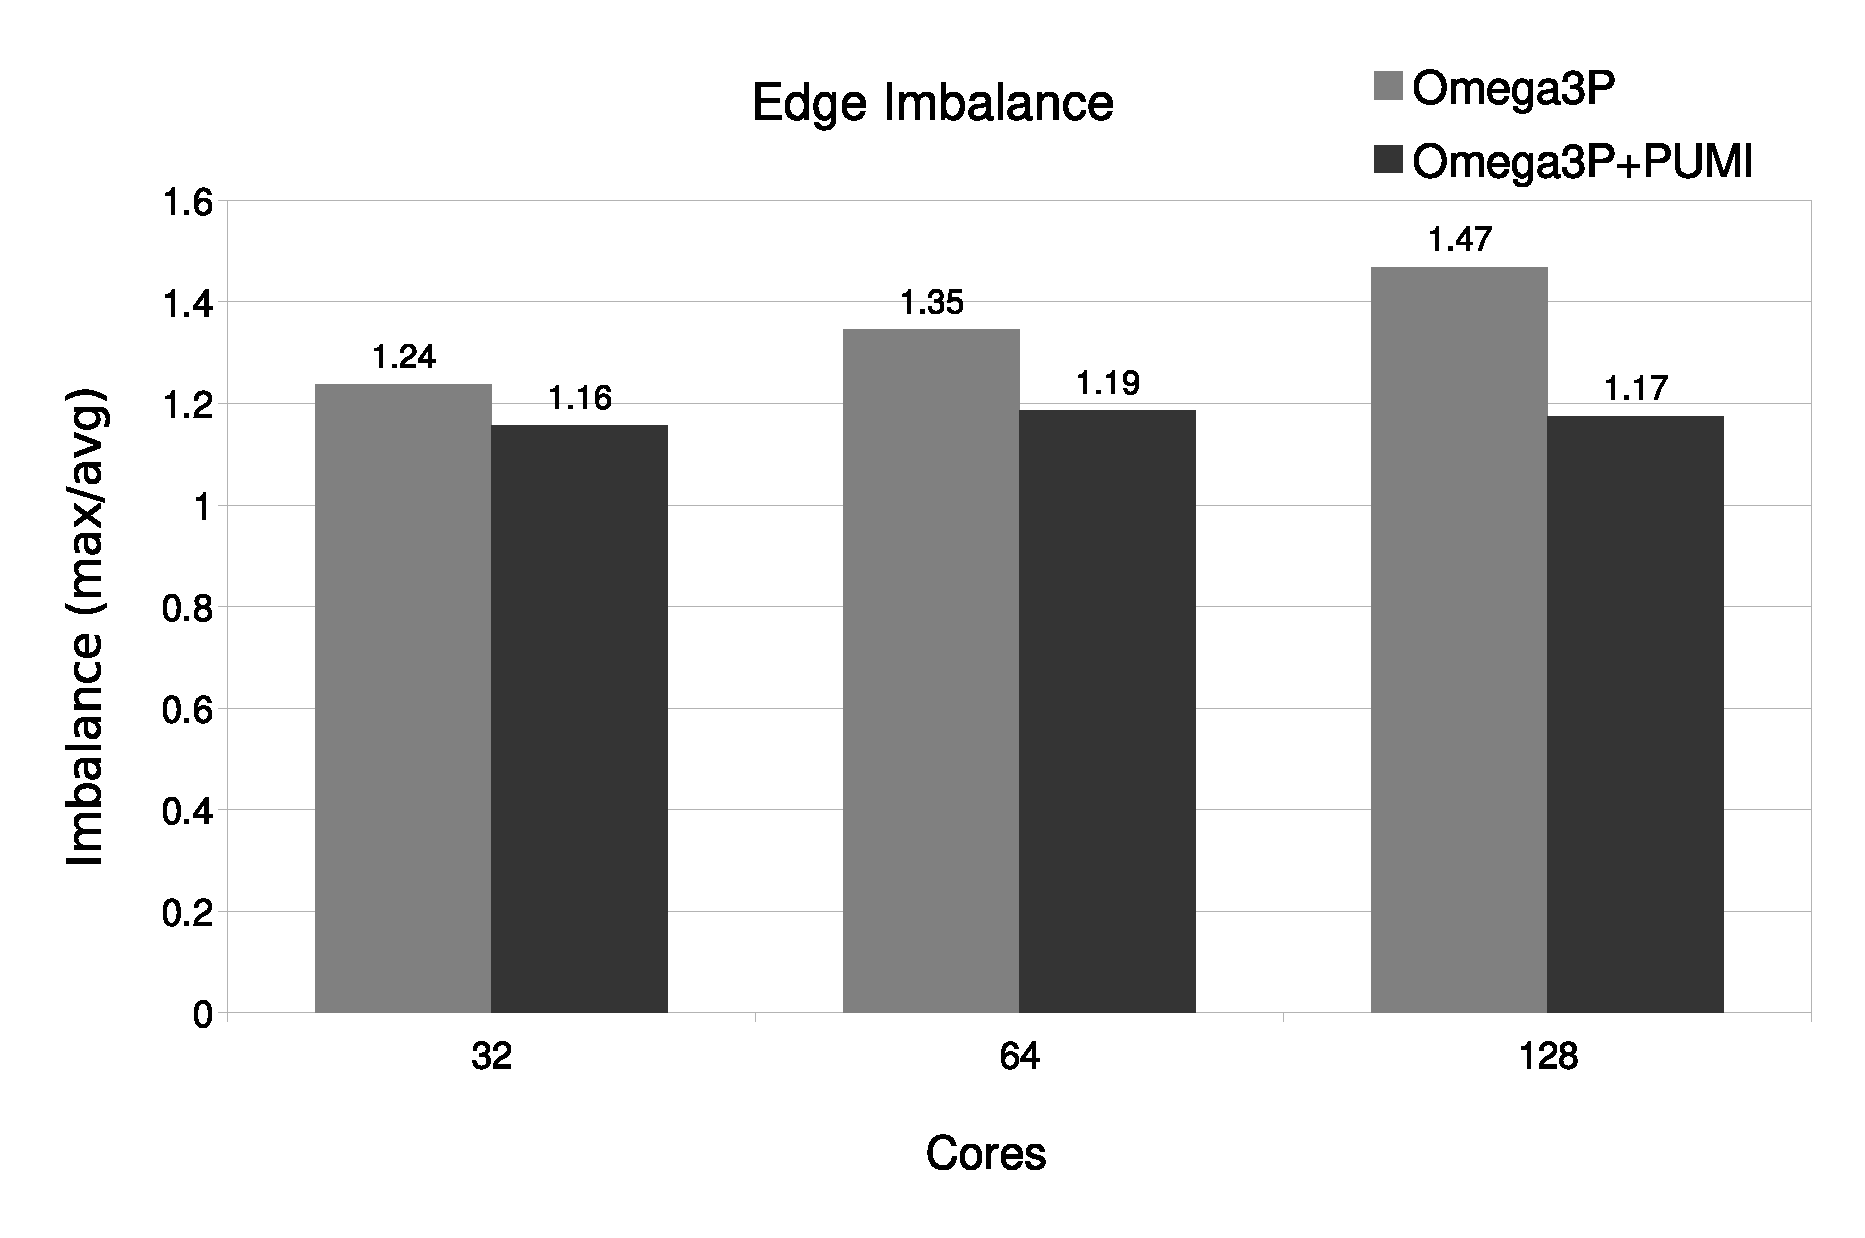
\includegraphics[width=\textwidth]{edge-imb.eps} \\
  \caption{\label{fig:vtx} Edge imbalance.}
\end{figure}

\begin{figure}[ht]
\centering
  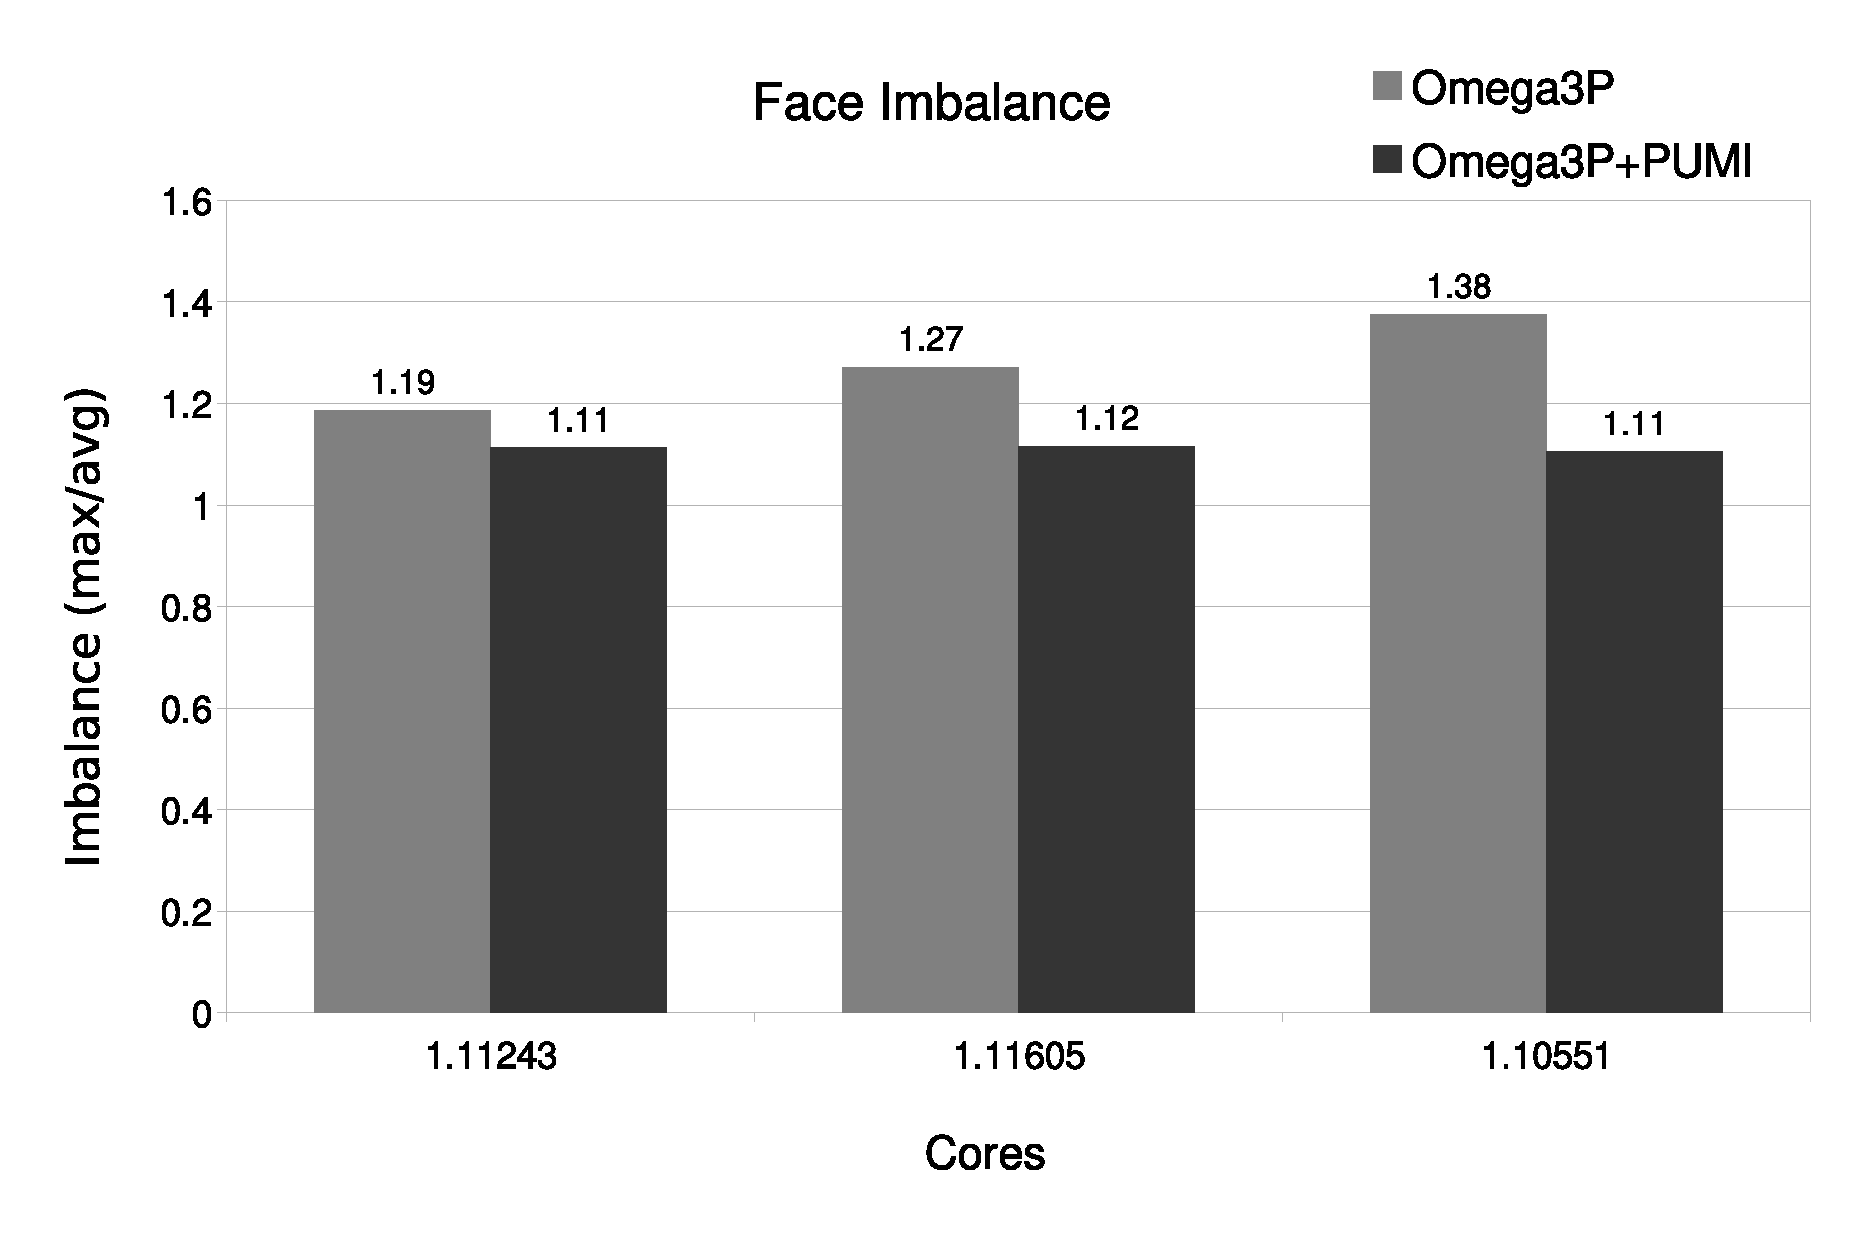
\includegraphics[width=\textwidth]{face-imb.eps} \\
  \caption{\label{fig:elm} Face imbalance.}
\end{figure}

Our next step is to perform a detailed analysis of the runtime and memory
usage.
After we have shown runtime improvements we plan to automate our regression
tests and work with SLAC developers to merge our changes into
the ACE3P central repository and make our documentation accessible.

To complete the adaptive loop we will begin work on solution-field transfer to
support mesh adaptation.
Critical to this work is determining where we will execute element level
integrals of the solution field.
We can either use Omega3P element integration routines, or implement the Nedelec
basis functions in our tensor-field component.
Reusing the Omega3P routines has the potential to reduce memory usage and code,
but may face difficulties near geometric model boundaries if parametric shape
information is not available.

\newpage \bibliographystyle{plain}
\bibliography{scorec-refs/partition,scorec-refs/meshdb,scorec-refs/hardware,scorec-refs/io,scorec-refs/frameworks,scorec-refs/cr,scorec-refs/fem,scorec-refs/meshgen}

\end{document}
